%-----------------------------------------------------------
%   Anexo A - Esquema elétrico
%-----------------------------------------------------------
\chapter{Esquema elétrico}
\label{anexo:EETS}

As páginas seguintes reproduzem as sete folhas do esquema elétrico da
unidade, geradas a partir de \texttt{hardware/gerador} (KiCad). O ficheiro
\texttt{Anexos/esquema\_eletrico.pdf} é copiado de
\texttt{hardware/laset\_gateway.pdf} sempre que o esquema muda.

\begin{enumerate}
    \item Alimentação: entrada de 5 a 60 V, LM5177 (5 V) e TPS62162 (3,3 V).
    \item Microcontrolador STM32H743ZIT6, oscilador, reset e SWD.
    \item Ethernet: LAN8742A e RJ45 com magnéticos.
    \item CAN FD: dois ADM3057E com terminação por jumper.
    \item RS485 (ADM2582E) e RS232 (MAX3227E).
    \item I2C com tradução de nível (PCA9306) e ligação ao GPS.
    \item PWM isolado (ADuM6401).
\end{enumerate}

\includepdf[pages=2-8,landscape,pagecommand={\thispagestyle{empty}}]{./Anexos/esquema_eletrico.pdf}
